\chapter{A ferramenta StarVZ} \label{ch:starvz}

Este Capítulo descreve em detalhes o \emph{Framework} StarVZ. Ele é 
apresentado genéricamente na Seção \ref{sect:starvz-overview}, a Seção 
\ref{sect:starvz-phases} apresenta de forma detalhadas as fases de sua 
execução, a Seção \ref{sect:related-work} disserta sobre otimizações já 
propostas e testadas e a Seção \ref{sect:motivation} fala sobre a motivação e a 
abordagem adotadas neste trabalho.

\section{Visão Geral}\label{sect:starvz-overview}
O StarVZ \cite{ref:starvz} é um \emph{workflow} de análise de performance cujo 
objetivo é auxiliar na avaliação e na verificação de hipóteses sobre a execução 
de 
aplicações \emph{task-based} em ambientes heterogêneos, executados sobre o
\emph{runtime} StarPU \cite{ref:starpu}. Ele é composto de duas fases, cada uma 
delas composta de uma combinação de diversas ferramentas, resultando em um 
\emph{framework}
rápido, consistente, flexível e versátil.

Na primeira fase, que pode ser visualizada na Figura 
\ref{fig:starvz-workflow1}, 
os 
\emph{Execution Traces} do StarPU, que são arquivos em um formato binário, são 
transformados
e exportados através da ferramenta \texttt{starpu\_fxt\_tool} para dois 
arquivos: DAG no formato DOT 
e Trace no formato PAJE. Essa etapa gera eventos com informação de data e hora, 
que 
descrevem o comportamento da aplicação para todos os recursos envolvidos. 
Também 
são gerados 
dados sobre o \emph{runtime} do StarPU, como número de tarefas submetidas,
número de tarefas prontas, arquitetura da plataforma, etc.

\begin{figure}[ht]
 \centerline{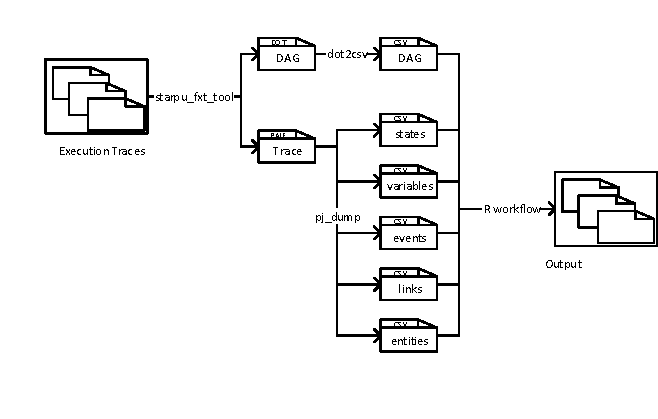
\includegraphics[width=1\textwidth]{./img/step1-final.pdf}}
 \caption{\emph{Workflow} de pré-processamento do StarVZ.}
 \label{fig:starvz-workflow1}
\end{figure}

Em seguida, é realizada uma verificação de integridade estrutural e temporal dos
arquivos \emph{trace}. Ela é executada via \texttt{pj\_dump}, gerando cinco 
arquivos: o arquivo states 
possui informações sobre as tarefas executadas e seu comportamento no 
\emph{runtime}; variables
consiste em métricas de performance da plataforma e \emph{runtime}; events 
possui informações sobre a 
utilização de recursos; links contém dados sobre comunicação MPI; e as 
informações de plataforma 
são registradas no arquivo entities. O DAG também passa por uma conversão e por 
fim, todos os 
arquivos são gravados no formato \emph{Comma-Separated Value} (CSV).

Finalmente, os dados escritos em CSV são lidos, filtrados, agregados e 
combinados em 
uma ferramenta implementada na linguagem R, utilizando-se bibliotecas oriundas 
do pacote 
\texttt{tidyverse} para a manipulação de dados. As saídas são escritas no 
formato \emph{FEATHER}
\cite{ref:feather}.

A segunda fase do \emph{workflow} inicia pela leitura das saídas da anterior. 
Cada arquivo
torna-se um \emph{data frame}, e os dados da execução inteira são unificados em 
uma estrutura.
É possível ter múltiplos \emph{traces} de aplicações sendo analisados em 
paralelo
para comparação, basta multiplicar a leitura com entradas diferentes e 
elas podem posteriormente ser combinadas em uma única visualização. A criação 
dos gráficos ainda 
possui processamento de dados, o que traz certa flexibilidade para as 
visualizações. Como última etapa dessa fase, o usuário 
parametriza o sistema com um arquivo de configuração no formato YAML, para que 
a 
montagem da visualização seja customizada. Finalmente, o usuário pode analisar 
os gráficos gerados pela ferramenta.

Nos experimentos realizados em \citet{ref:starvz}, em uma máquina equipada com 
um Intel(R) Xeon(R) 
CPU E3-1225 v3 @3.20GHz e 32GB de memória principal e com uma entrada de 
aproximadamente 18GB, a 
primeira fase do \emph{workflow} levou cerca de 32 minutos para executar: a 
execução da \texttt{starpu\_fxt\_tool}
levou em torno de 10 minutos, o \texttt{pj\_dump} levou cerca de 9 minutos e a 
ferramenta R levou cerca de 13
minutos. Já a segunda fase do \emph{workflow}, para executar a leitura dos 
arquivos \emph{FEATHER} e gerar
a visualização levou em torno de 2 minutos.

\section{Fases}\label{sect:starvz-phases}

\section{Trabalhos Relacionados}\label{sect:related-work}

O trabalho de \citet{ref:drakestarvz} foi o primeiro a tentar otimizar o fluxo 
do StarVZ. 
Sua principal motivação foi a melhoria de performance da etapa de manipulação 
de 
dados, a mais
custosa de acordo com os experimentos observados, com o objetivo de permitir o 
processamento de 
entradas maiores em um tempo aceitável.

Nele utilizou-se \texttt{Drake} \cite{ref:drake}, uma biblioteca para a 
linguagem de programação R, cujo foco é executar apenas as 
partes necessárias de um \emph{workflow} de análise de dados, evitando os 
passos 
desnecessários que não mudarão
suas saídas. Isso é realizado modelando as computações como um \emph{directed 
acyclic graph} (DAG) de tarefas e 
armazenando em cache os resultados daquelas já executadas. Além disso, 
\texttt{Drake} também possui suporte a paralelismo
(\emph{Implicit parallelism}) para a execução de tarefas independentes.

Para modelar o StarVZ dessa forma, foram necessárias mudanças cujo objetivo era 
explicitar 
dependências e postergar junções de \emph{data frames}. Depois da identificação 
dos fluxos independentes    
no \emph{workflow}, foi utilizado \texttt{Drake} para criar um plano de 
execução, que consiste na declaração
das tarefas onde cada uma é representada por uma função R. Na criação do plano, 
a biblioteca analisa cada
uma das tarefas, suas entradas e saídas, para determinar dependências e gerar o 
DAG. O resultado da modelagem do
StarVZ nessa abordagem pode ser visualizado na Figura \ref{fig:starvz-dag}.

\begin{figure}[ht]
\centerline{
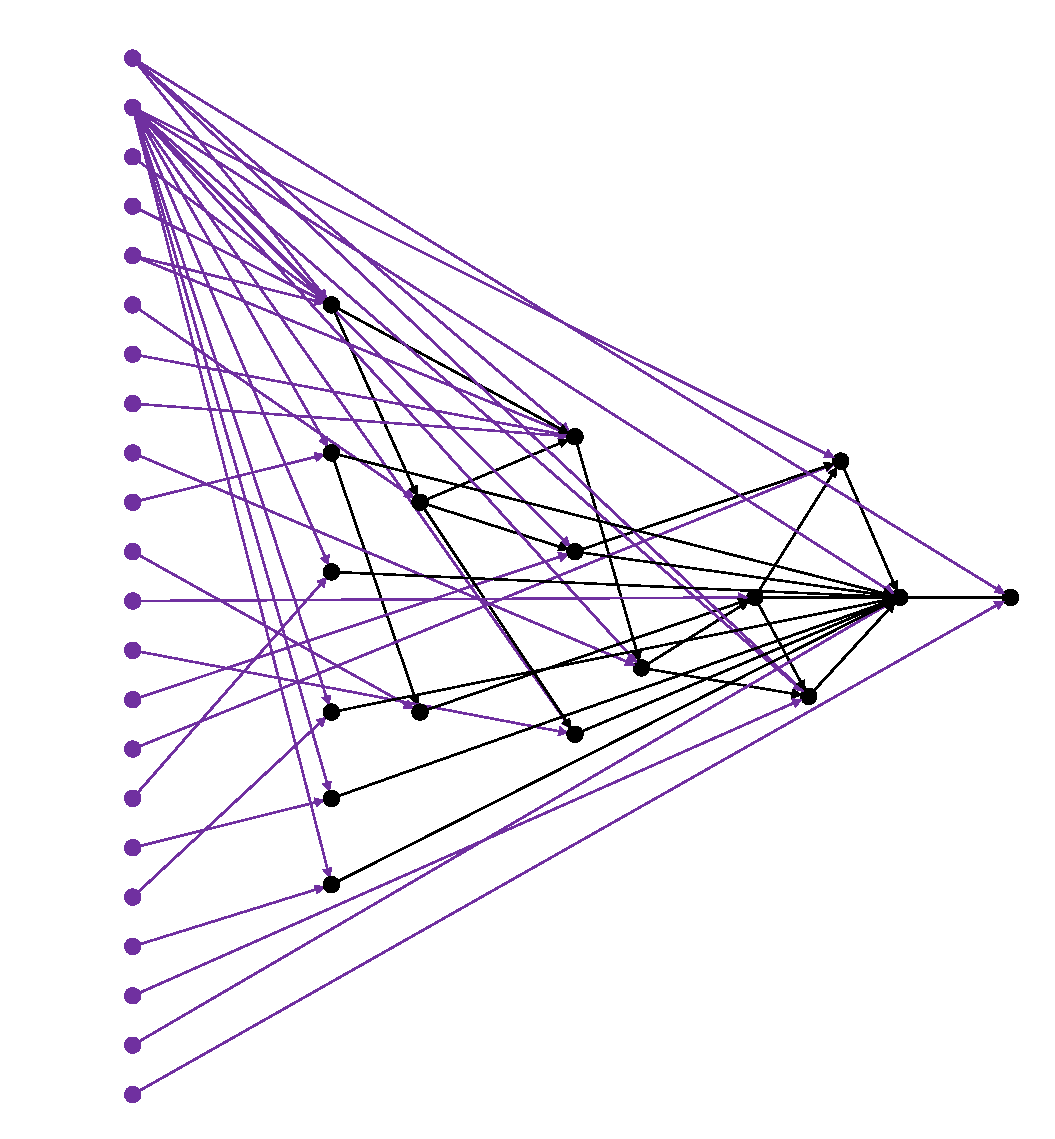
\includegraphics[width=0.8\textwidth]{./img/drake-dag-final-origin.pdf}}
 \caption{DAG de execução do StarVZ.}
 \legend{Fonte: Inspirada na Figura de contida no trabalho de 
\citet{ref:drakestarvz}}
 \label{fig:starvz-dag}
\end{figure}

Com esta modelagem, não foram observadas melhorias de performance no StarVZ. De 
acordo com \citet{ref:drakestarvz},
a cache de resultados intermediários da biblioteca acaba tendo que armazenar 
muitos dados em disco devido
ao tamanho dos \emph{data frames} gerados pelas entradas, prejudicando o tempo 
total de processamento.
Em relação ao suporte a paralelismo, ele é limitado pela falta de suporte 
nativo 
a \emph{multithread} da linguagem R.
Por isso, \texttt{Drake} oferece essa funcionalidade instanciando múltiplas 
sessões R, que são processos separados. A comunicação
entre esses processos é realizada pelo mesmo sistema de cache citado 
anteriormente, consequentemente, resultando nos mesmos
problemas.

Outra abordagem que poderia ser adotada para melhorar o desempenho do StarVZ 
seria distribuir os fluxos independentes
do \emph{workflow} pois elas podem trazer um ganho de desempenho em um ambiente 
viável.
Ao simplesmente paralelizar, é possível que os mesmo problemas com o tamanho 
dos 
\emph{data frames} sejam enfrentados, exigindo
máquinas com muita memória para obter-se os resultados desejados. 

A primeira opção seria distribuir os fluxos independentes utilizando o pacote 
\texttt{Snow}, que significa 
\emph{Simple Network of Workstations} \cite{ref:snow}. Este é desenvolvido para 
linguagem R e permite a utilização
de \emph{Explicit parallelism}, oferecendo integração com três interfaces de 
baixo nível: PVM (\emph{Parallel Virtual Machine}), através do pacote rpvm; 
MPI, 
através do pacote Rmpi \cite{ref:rmpi}; e uma integração com sockets, no caso 
de 
não ter nenhuma das outras 
opções disponíveis no ambiente. A utilização de \texttt{Snow} pode ser feita 
através da biblioteca \texttt{Snowfall} \cite{ref:snowfall},
que é um \emph{usability wrapper}, facilitando ainda mais a utilização.

A segunda alternativa seria a utilização da biblioteca \texttt{future} 
\cite{ref:future}. Esta provê uma forma simples e uniforme 
de avaliar expressões de forma assíncrona, utilizando recursos diversos. Ela 
funciona utilizando o conceito de abstração 
\emph{future}, que básicamente define um valor que poderá estar disponível no 
futuro. Tal valor pode ter seu estado como 
resolvido ou não resolvido, estado em que se ele for utilizado bloqueará o 
processo até sua resolução. Os \emph{futures} 
podem ser resolvidos de diversas formas: sequential, onde são resolvidos 
sequencialmente no processo R corrente; multiprocess,
que resolve utilizando \emph{multicore}; cluster, que é o mais interessante 
para 
adoção pois resolve com sessões R na máquina 
local e/ou em máquinas remotas; e etc.

\section{Motivação e Abordagem}\label{sect:motivation}
